\chapter{理论与技术支持}

本章将介绍区块链及云原生相关概念和理论知识, 还将介绍本文区块链云化框架所涉及到的其他技术与工具。

\section{区块链技术}\label{section: blockchain}

\subsection{区块链基本概念}
区块链是以比特币等数字加密货币体系为核心支撑技术的一种全新的去中心化基础架构与分布式计算范式\cite{1016383}。区块链通常被当作分布式账本, 具有去中心化、持久性、匿名性、不可篡改性、可追溯性的特点。

\begin{figure}[h] %figure环境,h默认参数是可以浮动,不是固定在当前位置。如果要不浮动,你就可以使用大写float宏包的H参数,固定图片在当前位置,禁止浮动。
    \centering %使图片居中显示
    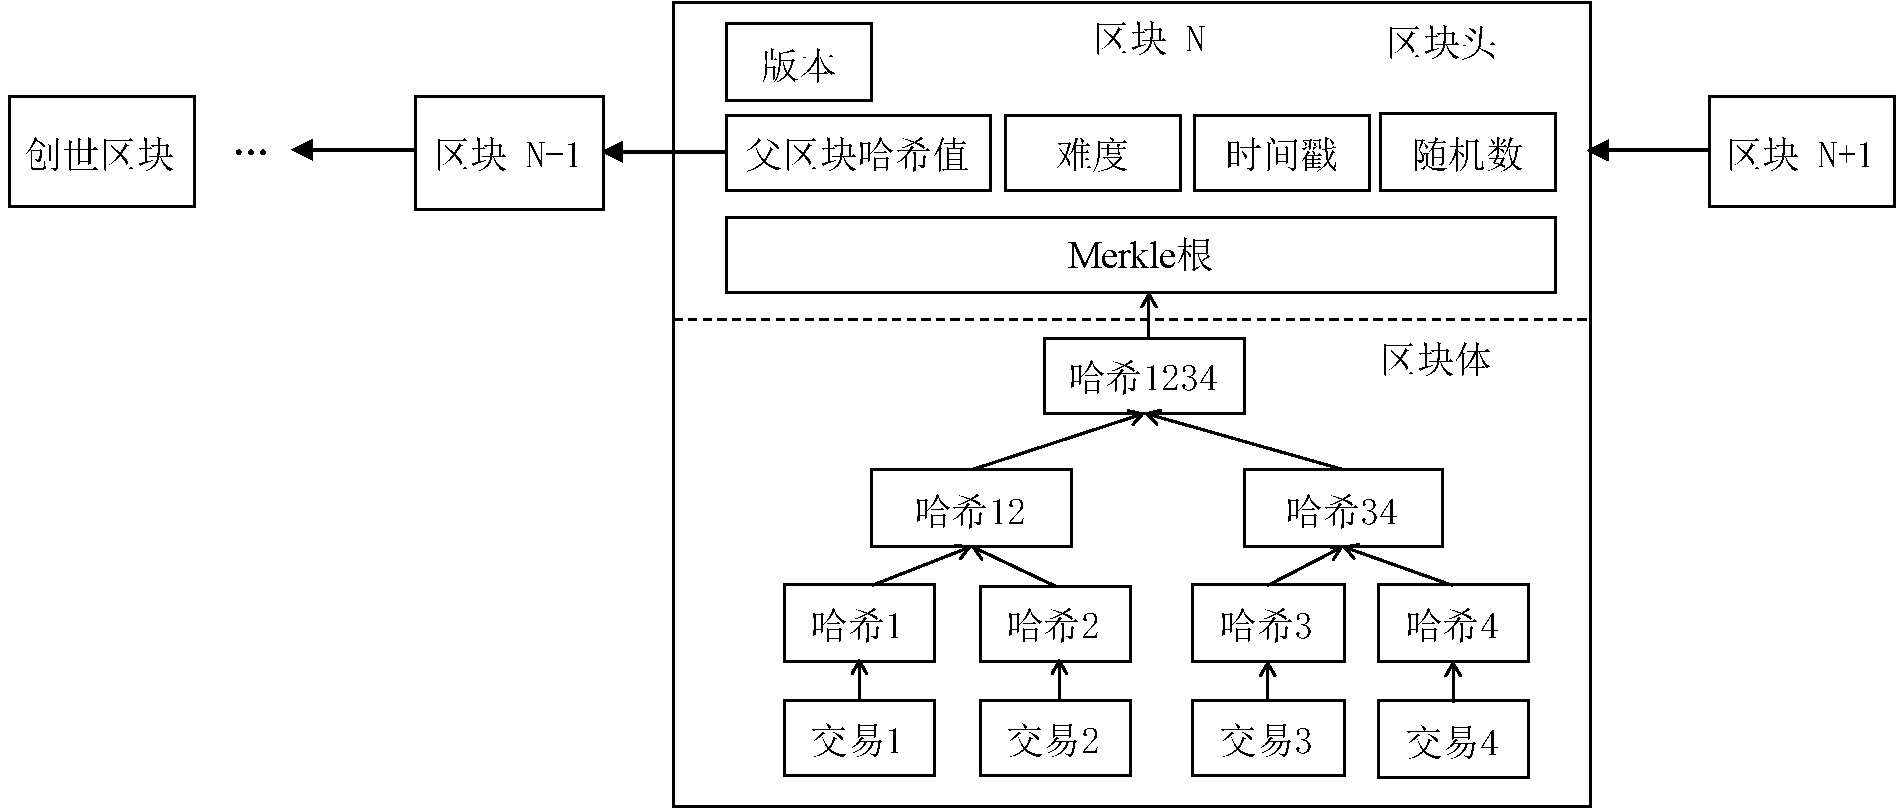
\includegraphics[width=1\textwidth]{FIGs/chapter2/blockchain_example.pdf} %中括号中的参数是设置图片充满文档的大小,你也可以使用小数来缩小图片的尺寸。
    \caption{区块链示例图} %caption是用来给图片加上图题的
    \label{blockchain_example} %这是添加标签,方便在文章中引用图片。
\end{figure}%figure环境

区块链典型示例如图\ref{blockchain_example}所示, 可以看作是一种按照时间顺序将数据区块以顺序相连的方式组合成的链式数据结构, 并以密码学方式保证其不可篡改和不可伪造。每个数据区块包含区块头(Block Header)和区块体(Block Body)两部分, 区块头主要用来存储本区块的一些相关属性, 区块体则用来存储真实的交易数据记录。区块头主要由三组数据组成, 第一组是父区块的哈希值, 用来将该区块与它的前一区块相连接; 第二组数据和矿工竞争挖矿有关, 即难度、时间戳和随机数(Nonce); 第三组是由区块体中计算出来的根哈希值, 即默克尔(Merkle)根。
区块体包括当前区块经过验证的、区块创建过程中生成的所有交易记录。这些记录通过默克尔树的哈希过程生成唯一的默克尔根并记入区块头。整个区块链的第一个区块称为创世区块(Genesis Block)。
如果网络中大多数节点就新区块中交易的有效性和区块本身的有效性达成共识, 则可以将新区块添加到链中。

{\footnotesize
\begin{longtable}[h]{m{70pt} m{70pt} m{70pt} m{70pt}}
    \caption[区块链类型]{区块链类型} \label{blockchain_type} \\
        \toprule   
        &\textbf{公有区块链}&\textbf{私有区块链}&\textbf{联盟区块链}\\
        \hline
        准入限制&无&有&有\\
        
        读取者&任何人&仅限受邀用户&相关联用户\\
        
        写入者&任何人&获批参与者&获批参与者\\
        
        所属者&无&单一实体&多方实体\\
        
        交易速度&慢&快&快\\
        \bottomrule
    \end{longtable}
}

当前, 区块链分为公有区块链、联盟区块链和私有区块链。如表\ref{blockchain_type}所示, 公有链没有准入限制, 没有监管方参与, 任何人都可以参与共识, 常见的两种共识协议为工作量证明机制(Proof of Work, 简称PoW)和权益证明机制(Proof of Stake, 简称PoS)。公有链允许任何人都可以自由加入, 具有高度分布式的拓扑结构。但是, 公有链在安全性和性能方面也进行了权衡。公有链上的许多服务器遇到了扩展瓶颈, 吞吐量相对较弱; 与公有区块链的无准入限制形成鲜明对比的是, 私有区块链建立了准入规则, 规定谁可以查看和写入区块链。因为在控制方面有明确的层次结构, 私有链也不是去中心化系统。在某些私有链中, 具备安全模型的背景下, 共识协议是多余的。因此在私有区块链中, 不使用PoW并不会造成很严重的威胁, 因为每个参与者的身份都是已知的, 是手动进行管理的; 联盟区块链是介于公有链和私有链之间的, 结合了两者的特征要素。在共识方面, 联盟链将少数同等权力的参与方视为验证者, 而不是像公有链那样开放的系统, 让任何人都可以验证区块, 也不是像私有链那样, 通过一个封闭的系统, 只允许某一个实体来任命区块的生产者。对于从事各类活动的个人和企业来说, 存在大量的区块链选择。即使在公有链、私有链和联盟链中, 根据复杂性的不同, 也会出现许多不同的用户体验。根据实际使用情况, 企业可以选择最适合的链实现目标产品。供应链、电商、医疗等需要彼此之间相互沟通的场景下, 联盟链可减轻私有链中交易对手的风险, 并且较少的节点数通常可使它们能够比公有链更有效率。

\subsection{Hyperledger Fabric}
Hyperledger Fabric\footnotemark[1]\footnotetext[1]{\href{https://github.com/hyperledger/fabric}{Hyperledger Fabric}}是一种企业级联盟链解决方案, 因其可插拔模块化、可伸缩、可扩展的架构、多编程语言的智能合约受到业界广泛追捧。

\begin{figure}[h] %figure环境,h默认参数是可以浮动,不是固定在当前位置。如果要不浮动,你就可以使用大写float宏包的H参数,固定图片在当前位置,禁止浮动。
    \centering %使图片居中显示
    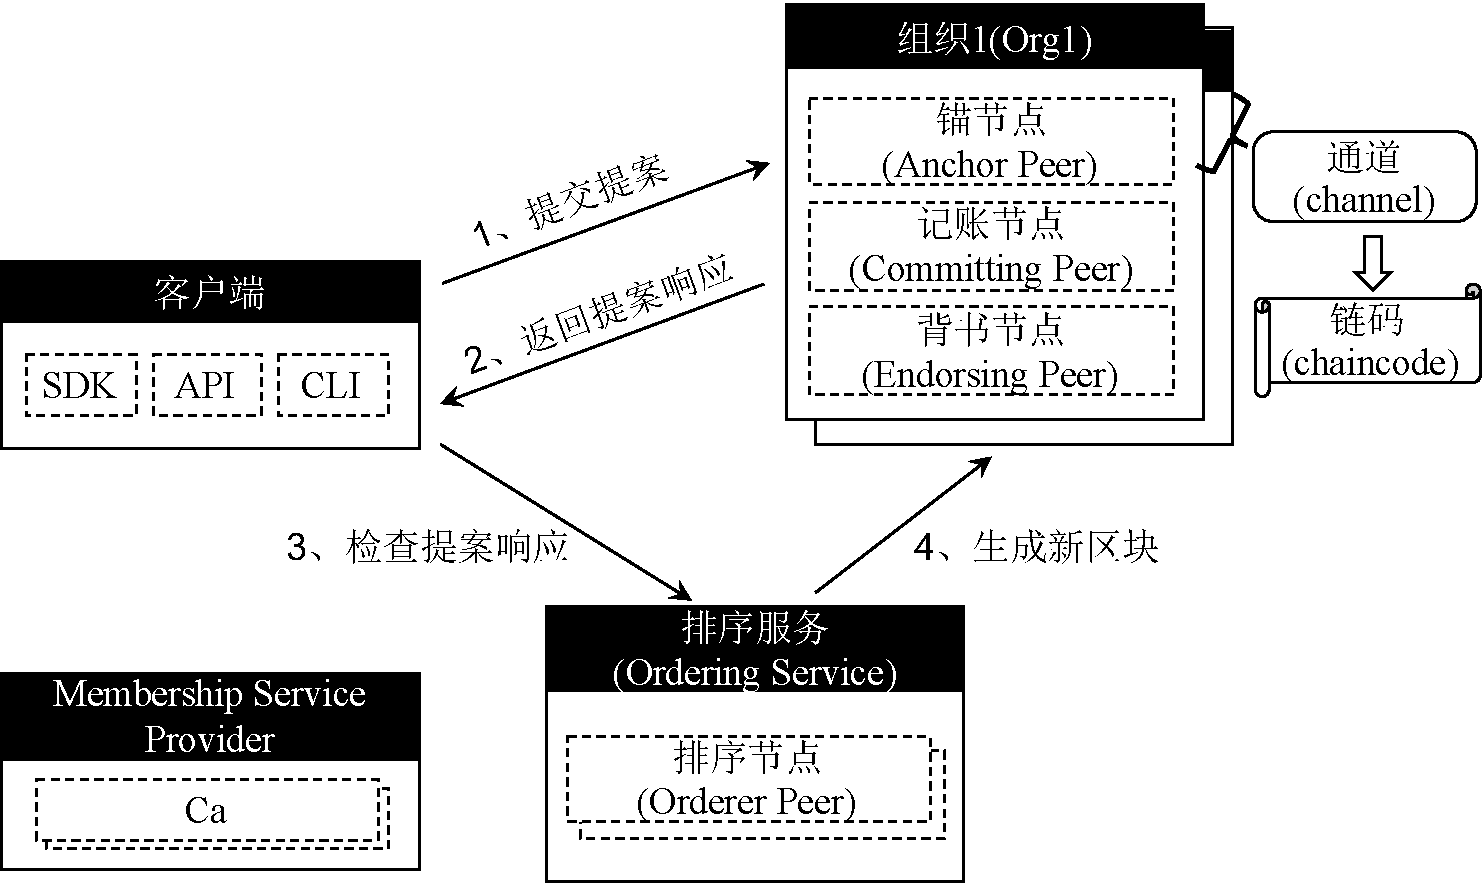
\includegraphics[width=1\textwidth]{FIGs/chapter2/hyperledger_fabric.pdf} %中括号中的参数是设置图片充满文档的大小,你也可以使用小数来缩小图片的尺寸。
    \caption{Hyperledger Fabric网络架构} %caption是用来给图片加上图题的
    \label{hyperledger_fabric} %这是添加标签,方便在文章中引用图片。
\end{figure}%figure环境 

如图\ref{hyperledger_fabric}所示, HF网络通过组织划分, 每个组织内包含多种不同角色的Peer节点, 每个Peer节点又可以担任多种角色, 所有的组织共用排序服务。HF多种节点通过网络相互链接组成联盟链网络完成链上交易。

\textbf{网络节点}
\begin{enumerate}[fullwidth,itemindent=2em,label=(\arabic*)]
    \item 客户端节点: 在HF网络外部用于主动与区块链交互、实现区块链操作的组件。常见的客户端节点有软件开发工具包(Software Development Kit, 简称SDK)\footnotemark[2]\footnotetext[2]{\href{https://github.com/hyperledger/fabric-sdk-go}{Hyperledger Fabric Go版本的SDK}}、Fabric-CLI\footnotemark[3]\footnotetext[3]{\href{https://github.com/hyperledger/fabric-cli}{fabric cli}}、REST API\footnotemark[4]\footnotetext[4]{\href{https://github.com/hyperledger/fabric/blob/v0.6/docs/source/API/CoreAPI.rst}{fabric api}};

    \item Ca节点: Fabric-Ca\footnotemark[5]\footnotetext[5]{\href{https://github.com/hyperledger/fabric-ca}{fabric ca}}是一个官方可选的Membership Service Provider(MSP)组件, 对HF网络中各实体(Identity)的数字身份证书进行管理。完成实体身份注册、数字证书的签发续签或吊销;

    \item Peer节点: HF网络的每个组织都包含一个或多个Peer节点, 每个Peer节点可以通过配置文件担任一种或多种角色。

    \begin{itemize}[itemindent=2em]
        \item 锚节点(Anchor Peer): 负责与其他组织的锚节点进行通信;

        \item 记账/提交节点(Committing Peer): 负责对区块及区块交易进行验证, 验证通过后将区块写入账本中, 同时提交节点会定期与其他节点通过Gossip协议进行信息交换;

        \item 背书节点(Endorsing Peer): 负责对客户端发送的提案进行签名背书。背书节点与具体的链码(Chaincode)绑定, 其通过调用链码模拟执行交易并向生成提案的客户端返回提案响应。背书节点是动态的, 在客户端发起提案时才会根据背书策略(Endorsement Policy)成为背书节点, 其他时候为记账节点。
    \end{itemize}

    \item Orderer节点: 排序服务节点接收经过背书签名的交易并对未打包的交易进行排序生成新区块, 最终通过原子广播到记账节点。排序服务采取可插拔设计, 支持Solo、Kafka等分布式共识协议。

\end{enumerate}

HF区块链支持在通信节点之间启用传输层安全性协议(Transport Layer Security, 简称TLS)保证两通信节点的数据保密性和完整性。TLS采用x509证书进行身份验证并生成会话密钥, 不仅支持客户端节点对服务节点的身份验证, 同时也支持服务节点来验证客户端的双向验证。

\textbf{账本结构}

HF中智能合约被称为链码, 通过通道(Channel)允许参与者同时履行不同的链码。HF网络子链通常按照“1个通道+1个账本+N个成员”组成。不同组织及其成员能够在通道中完成特定的交易, 限制信息传播范围。建立一个通道就相当于创建了一条子链, 这条子链上只拥有唯一的一份账本。

\begin{figure}[h] %figure环境,h默认参数是可以浮动,不是固定在当前位置。如果要不浮动,你就可以使用大写float宏包的H参数,固定图片在当前位置,禁止浮动。
    \centering %使图片居中显示
    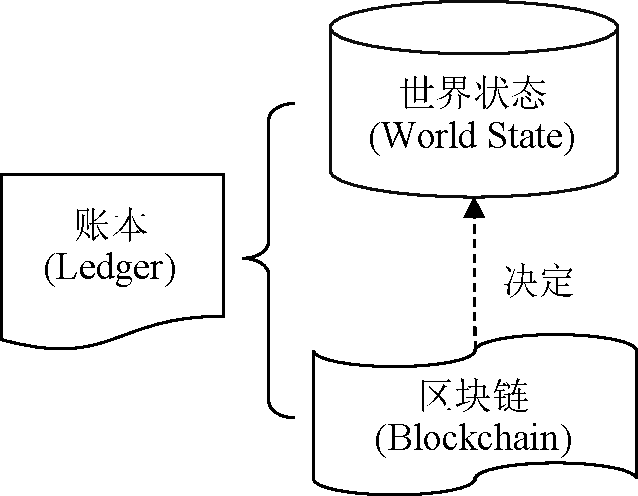
\includegraphics[width=0.45\textwidth]{FIGs/chapter2/ledger.pdf} %中括号中的参数是设置图片充满文档的大小,你也可以使用小数来缩小图片的尺寸。
    \caption{Hyperledger Fabric账本结构} %caption是用来给图片加上图题的
    \label{fabric_ledger} %这是添加标签,方便在文章中引用图片。
\end{figure}%figure环境

如图\ref{fabric_ledger}所示, HF账本由区块链以及世界状态(World State)组成, 其中世界状态由区块链决定。
首先, 世界状态是一个可插拔的键值对(Key-Value, 简称K-V)数据库, 提供简单、快速、丰富的账本状态检索和存储方式。通过世界状态, 客户端能够直接定位访问账本状态的某个值, 不需要遍历计算整个交易日志。为解决不同类型的问题, HF提供了LevelDB和CouchDB来保障账本状态类型的灵活性。当账本状态是简单的键值对时, 使用LevelDB合适; 当账本状态结构为 JSON时, 使用CouchDB合适。
其次, 这里的区块链指的是交易日志, 不是指区块形成的链。区块记录了世界状态改变的历史, 并以文件的方式进行持久化。交易数据一旦写入区块链就无法篡改。

\subsection{Blockchain as a Service}\label{section: BaaS}

\begin{figure}[h] %figure环境,h默认参数是可以浮动,不是固定在当前位置。如果要不浮动,你就可以使用大写float宏包的H参数,固定图片在当前位置,禁止浮动。
    \centering %使图片居中显示
    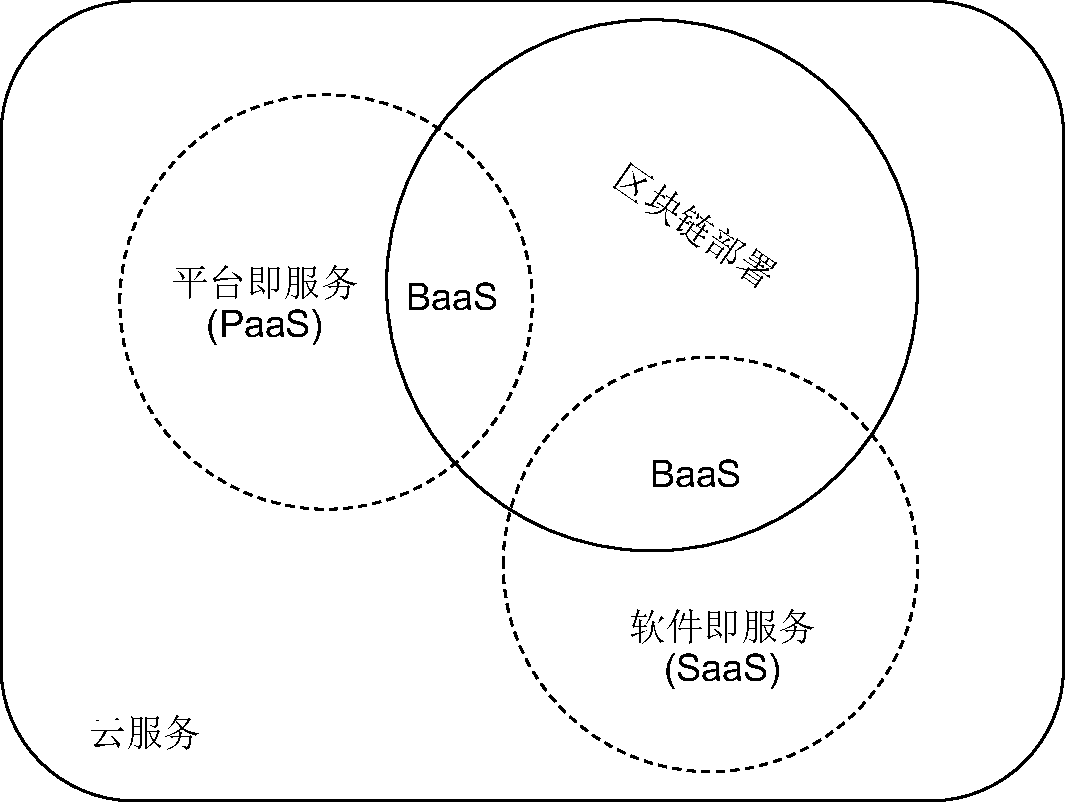
\includegraphics[width=0.55\textwidth]{FIGs/chapter2/BaaS_PaaS_SaaS.pdf} %中括号中的参数是设置图片充满文档的大小,你也可以使用小数来缩小图片的尺寸。
    \caption{BaaS与PaaS以及SaaS的对比} %caption是用来给图片加上图题的
    \label{BaaS_PaaS_SaaS} %这是添加标签,方便在文章中引用图片。
\end{figure}%figure环境

随着区块链以及云原生的发展, BaaS也悄然兴起。云提供了一种按需的、虚拟的、资源可伸缩的IT环境, BaaS则提供了一种基于云的区块链服务。BaaS能够在云上构建、管理、托管和运维区块链技术, 能够快速部署区块链网络及其开发环境、编写智能合约、构建去中心化应用(即区块链应用, Decentralized Application, 简称 Dapp)。基于云基础设施, BaaS屏蔽了底层区块链与云原生的逻辑, 消除了用户构建开发去中心化应用的壁垒, 为用户提供便捷的、一体化的区块链的能力。如图\ref{BaaS_PaaS_SaaS}所示, 根据BaaS的实施方式, BaaS在云环境中的位置会有所不同\cite{onik2019performance}。BaaS可以从平台即服务(Platform as a Service, 简称PaaS)获得基础设施支持的同时也可以从软件即服务(Software as a Service, SaaS)获得软件服务。

微软推出由Azure云驱动的开放式区块链平台Bletchley, 该项目保证服务对于所有平台、合作者和客户来讲都是开放的、灵活的\cite{BlockchainasaServiceNextGenerationofCloudServices}。IBM推出了名为Bluemix的云计算平台, 依托于PaaS云帮助开发者更快地进行应用开发和部署。随后AWS、Google、阿里云等也相继推出自家的区块链即服务平台。以HF为例, BaaS平台通用的架构如\ref{BaaS_Architecture}所示, 本质上BaaS以计算、存储等资源为基础, 联合上层的区块链基础设施的相关能力, 如共识能力、记账能力、智能合约等转化为可编程接口, 使得区块链网络的部署以及去中心化应用开发过程简单而高效。同时, BaaS通过底层标准化的云基础设施能力为上层的区块链及其去中心化应用提供安全可靠的支撑, 解决弹性、网络、安全性、性能等难题。本文重点关注于基础设施层中Kubernetes上的区块链云化框架的研究。

\begin{figure}[h] %figure环境,h默认参数是可以浮动,不是固定在当前位置。如果要不浮动,你就可以使用大写float宏包的H参数,固定图片在当前位置,禁止浮动。
    \centering %使图片居中显示
    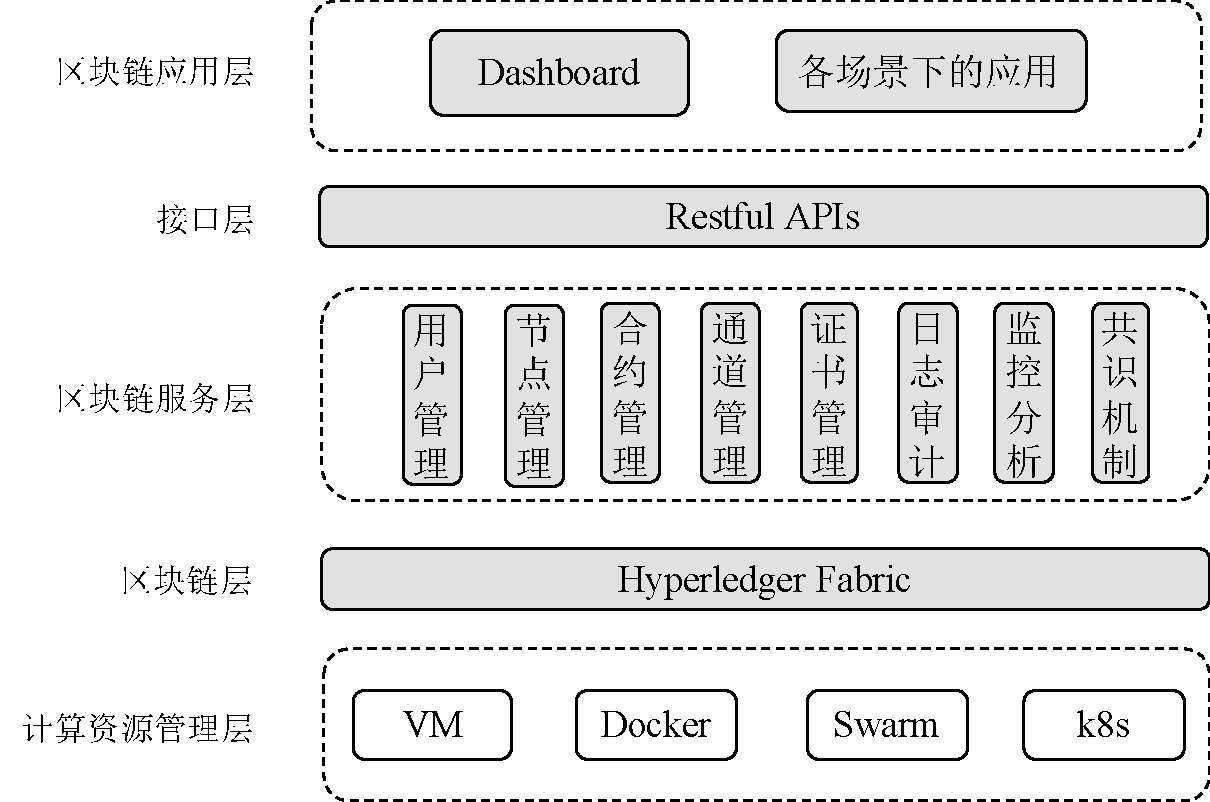
\includegraphics[width=0.85\textwidth]{FIGs/chapter2/BaaS_Architecture.pdf} %中括号中的参数是设置图片充满文档的大小,你也可以使用小数来缩小图片的尺寸。
    \caption{BaaS通用架构} %caption是用来给图片加上图题的
    \label{BaaS_Architecture} %这是添加标签,方便在文章中引用图片。
\end{figure}%figure环境

\section{云原生}\label{section: cloud_native}

\subsection{云原生基本概念}

云原生, 即云原生计算。从发展历程来说, 云原生是云计算的升级。云计算最早由Dell公司在1996年提出\cite{ZHANG20121791}, 亚马逊公司在2006年率先推出的弹性计算云(Elastic Compute Cloud, 简称EC2)服务对云计算产生了深刻影响, 越来越多的企业开始逐步接受云计算这一概念, 并将应用逐步迁移到云端, 享受这一新型计算方式带来的技术红利。此后, 软件系统规模、软件开发方式驱动着技术不断升级。在云计算的时代, 云端只是用于计算的场所, 应用无须重新编写, 只需重新部署, 应用的迁移从物理机到虚拟机, 存储选用兼容的块存储或文件存储。但几乎所有分布式场景中都需应用自行解决稳定性、数据同步、容灾等方面的问题。要解决这些问题, 只能从根本上寻求解决方案。即从迁移到云转变为诞生于云。2013年Docker开源, 之后Pivotal公司提出了云原生的概念, 这是对云计算概念的全面升级。Pivotal指出云原生由容器、微服务、DevOps以及持续交付等技术\cite{WhatisCloudNative}组成, 并充分利用云计算优势构建和运行应用。2014年, 容器编排技术Kubernetes发布。容器技术日趋成熟, 在业界开始广泛应用。在2015年, 
云原生计算基金会(Cloud Native Computing Foundation, 简称CNCF)成立。而到了2021年, CNCF已经孵化了超过120个项目、740名成员以及142000的贡献者\footnotemark[1]\footnotetext[1]{\href{https://www.cncf.io/wp-content/uploads/2022/01/CNCF_Annual_Report_2021.pdf}{CNCF2021年年度报告}}。除了工业界, 云原生在学术界也引起了关注, 《计算机学报》发起了以“云原生”为主题的专刊征文\footnotemark[2]\footnotetext[2]{\href{http://chinasoft.ccf.org.cn/papers/7.html}{《计算机学报》云原生软件技术与工程实践专刊征文通知-CCF2021中国软件大会}}。

\begin{figure}[h] %figure环境,h默认参数是可以浮动,不是固定在当前位置。如果要不浮动,你就可以使用大写float宏包的H参数,固定图片在当前位置,禁止浮动。
    \centering %使图片居中显示
    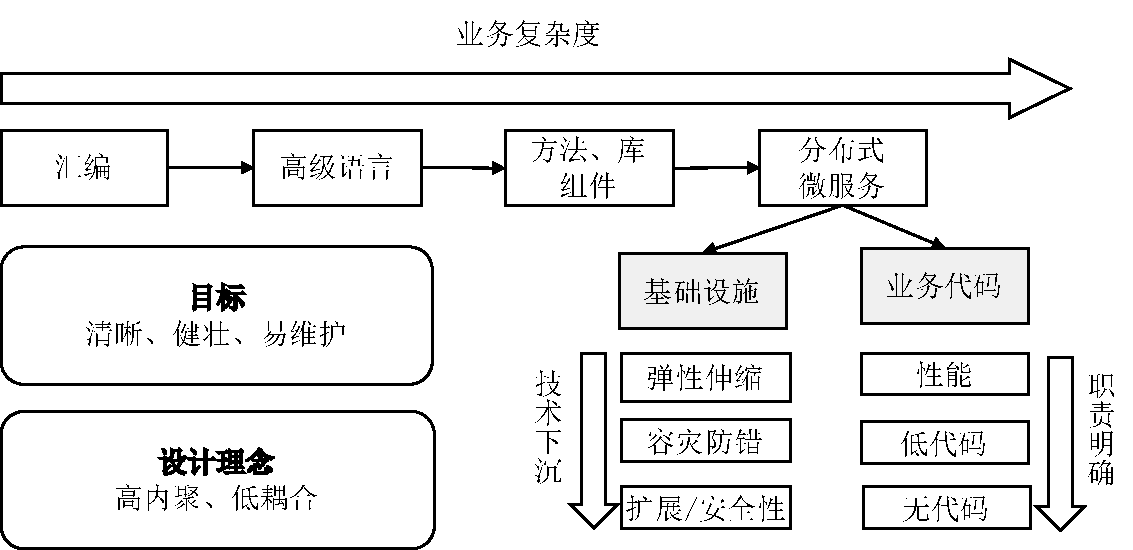
\includegraphics[width=0.9 \textwidth]{FIGs/chapter2/cloud_native_development.pdf} %中括号中的参数是设置图片充满文档的大小,你也可以使用小数来缩小图片的尺寸。
    \caption{云原生技术发展趋势} %caption是用来给图片加上图题的
    \label{cloud_native_development} %这是添加标签,方便在文章中引用图片。
\end{figure}%figure环境

以软件工程的视角来看, 如图\ref{cloud_native_development}所示, 随着软件规模、软件复杂程度在不断增大, 软件上线速度不断加快, 软件稳定性的要求在不断提高。围绕着“高内聚、低耦合”的设计理念, 软件制品进一步深层次抽象, 从单体架构演化为分布式微服务架构, 从可复用的方法、库、组件进一步下沉到底层的基础设施。在这些客观需求的驱动下, 敏捷进一步向运维端延伸, 继瀑布开发、敏捷开发之后, 开发运维一体化(Development and Operations, 简称DevOps)成为又一新兴的软件开发理念和愿景。由于软件体量巨大, 多个不同职责明确的团队负责整体软件项目的运行。DevOps旨在通过一系列文化及技术手段(尤其是自动化IT工具链)打破开发和运维团队之间的壁垒, 改善团队之间的协作关系, 实现更加频繁快速、可靠的软件产品交付\cite{ChinaDevops}。DevOps不仅向运维端扩展, 其更涉及到软件全生命周期中的人、流程与平台。可以说, DevOps是当下软件工程的第一生产力, 其是一种普世的价值观。云原生作为一种基于云基础设施的技术体系涵盖了云应用定义、开发、构建与运行时的所涉及到的各工具或平台。云原生是DevOps生产力下的现阶段生产工具的体现, 是DevOps 的价值具象, “DevOps 时代下的云原生”就如“蒸汽时代的蒸汽机”。

\begin{figure}[h] %figure环境,h默认参数是可以浮动,不是固定在当前位置。如果要不浮动,你就可以使用大写float宏包的H参数,固定图片在当前位置,禁止浮动。
    \centering %使图片居中显示
    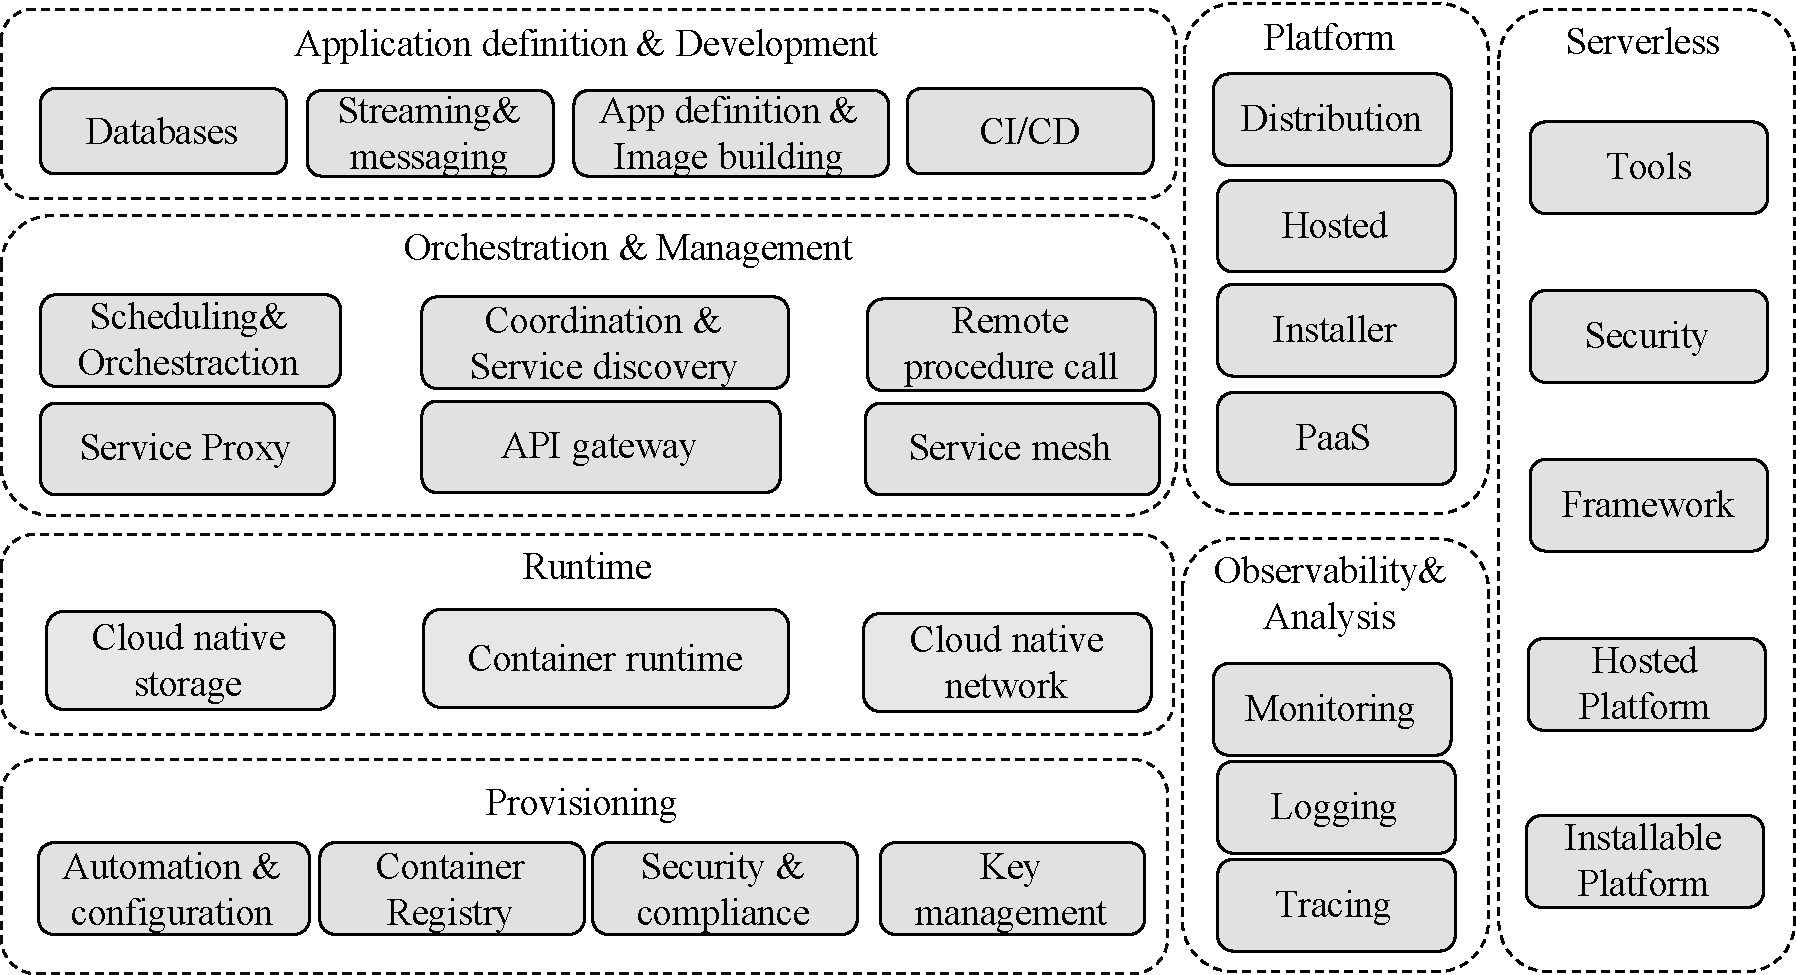
\includegraphics[width=1.0 \textwidth]{FIGs/chapter2/cloud_native_landscape.pdf} %中括号中的参数是设置图片充满文档的大小,你也可以使用小数来缩小图片的尺寸。
    \caption{云原生技术范畴} %caption是用来给图片加上图题的
    \label{cloud_native_landscape} %这是添加标签,方便在文章中引用图片。
\end{figure}%figure环境

云原生技术囊括了DevOps的各环节。如图\ref{cloud_native_landscape}所示, CNCF定义了云原生的技术范畴, 主要包括: 

\begin{itemize}[itemindent=2em]
    \item 供应层(Provisioning): 涉及云原生应用运行环境的自动化基础设施;

    \item 运行时(Runtime): 指保障云原生应用程序正常运行所需的沙盒;

    \item 云应用编排与管理(Orchestration and Management): 为云原生应用提供自动化编排和弹性伸缩能力, 让云原生应用天然地具备可扩展性;

    \item 云应用定义与开发(Application Definition and Development): 开发、构建、部署和运行应用程序的工具;

    \item 可观测性与分析(Observability and Analysis): 全方位监控和分析云原生应用层的工具;

    \item 平台(Platform): 主要指Kubernetes, 将多类工具有机组合在一起解决庞大的工程问题;

    \item 无服务器(Serverless): 提供函数级别更细粒度部署的一种新的云原生计算模型。
\end{itemize}


随着云架构的不断普及,“未来的软件一定生长于云上”的理念被越来越多的人所接受。云提
供了一种面向企业应用按需进行资源分配的模型, 以一种全新的高效的方式来部署应用。云原生是一系列基于云技术体系和企业管理方法的集合, 既包含了实现应用云原生化的方法论, 也包含了落地实践的关键技术。云原生应用利用容器、服务网格、微服务、不可变基础设施和声明式API等代表性技术, 来构建容错性好、易于管理和便于观察的松耦合系统, 结合可靠的自动化手段可对系统做出频繁、可预测的重大变更, 让应用随时处于待发布状态。Gartner指出, 到2022年全球公共云服务市场预计将增长至约3546亿美元, 60\%的组织将使用外部服务提供商的云管理服务\cite{bhagavan2020achieving}。企业纷纷开始云化转型, 希望将传统应用迁移到云端。

\begin{figure}[h] %figure环境,h默认参数是可以浮动,不是固定在当前位置。如果要不浮动,你就可以使用大写float宏包的H参数,固定图片在当前位置,禁止浮动。
    \centering %使图片居中显示
    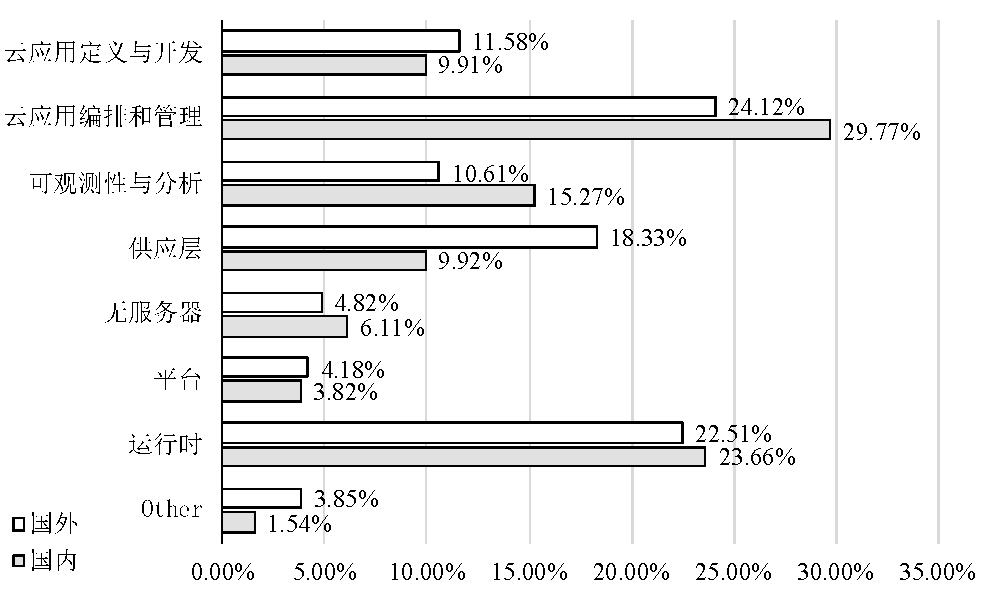
\includegraphics[width=0.9 \textwidth]{FIGs/chapter2/workshop.pdf} %中括号中的参数是设置图片充满文档的大小,你也可以使用小数来缩小图片的尺寸。
    \caption{国内外云原生技术现状} %caption是用来给图片加上图题的
    \label{workshop} %这是添加标签,方便在文章中引用图片。
\end{figure}%figure环境

如图\ref{workshop}所示, 本文根据上述7类云原生技术范畴, 对2020-2021年国内外重点技术会议的共442场分享进行了系统化分析, 其中包括国内云原生社区MeetUp城市站以及Cloud Native+Open Source Virtual Summit China共131场分享, 国际(欧洲、北美)KubeCon+CloudNativeCon Europe以及KubeCon+CloudNativeCon North America 共311篇场分享。从表中可知, 目前国内外研究重点关注于云应用编排以及运行时, 国内对云应用编排与管理的讨论要大于国际并且云应用定义与开发流程、可观测性与分析、平台与无服务器方面国内外相关分享在比例上差距并不是很大, 云原生技术体系已经成为当代软件工程技术发展的主流技术体系。

\subsection{Kubernetes}

Kubernetes(简称k8s)是Google开源的容器集群管理平台。在容器化技术之上, Kubernetes为容器化的云原生应用提供部署运行、资源调度、服务发现、弹性伸缩等一系列基础功能, 提升了大规模容器集群管理的便捷性。自开源来, Kubernetes成为一种全新的基于容器技术的分布式架构解决方案, 在云原生领域具有举足轻重的地位。2019年, 在我国72\%的工程师已经在云原生生产环境中大规模使用Kubernetes\footnotemark[1]\footnotetext[1]{\href{https://www.cncf.io/blog/2020/10/13/cncf-cloud-native-survey-china-2019/}{CNCF Cloud Native Survey China 2019}}。

\begin{figure}[h] %figure环境,h默认参数是可以浮动,不是固定在当前位置。如果要不浮动,你就可以使用大写float宏包的H参数,固定图片在当前位置,禁止浮动。
    \centering %使图片居中显示
    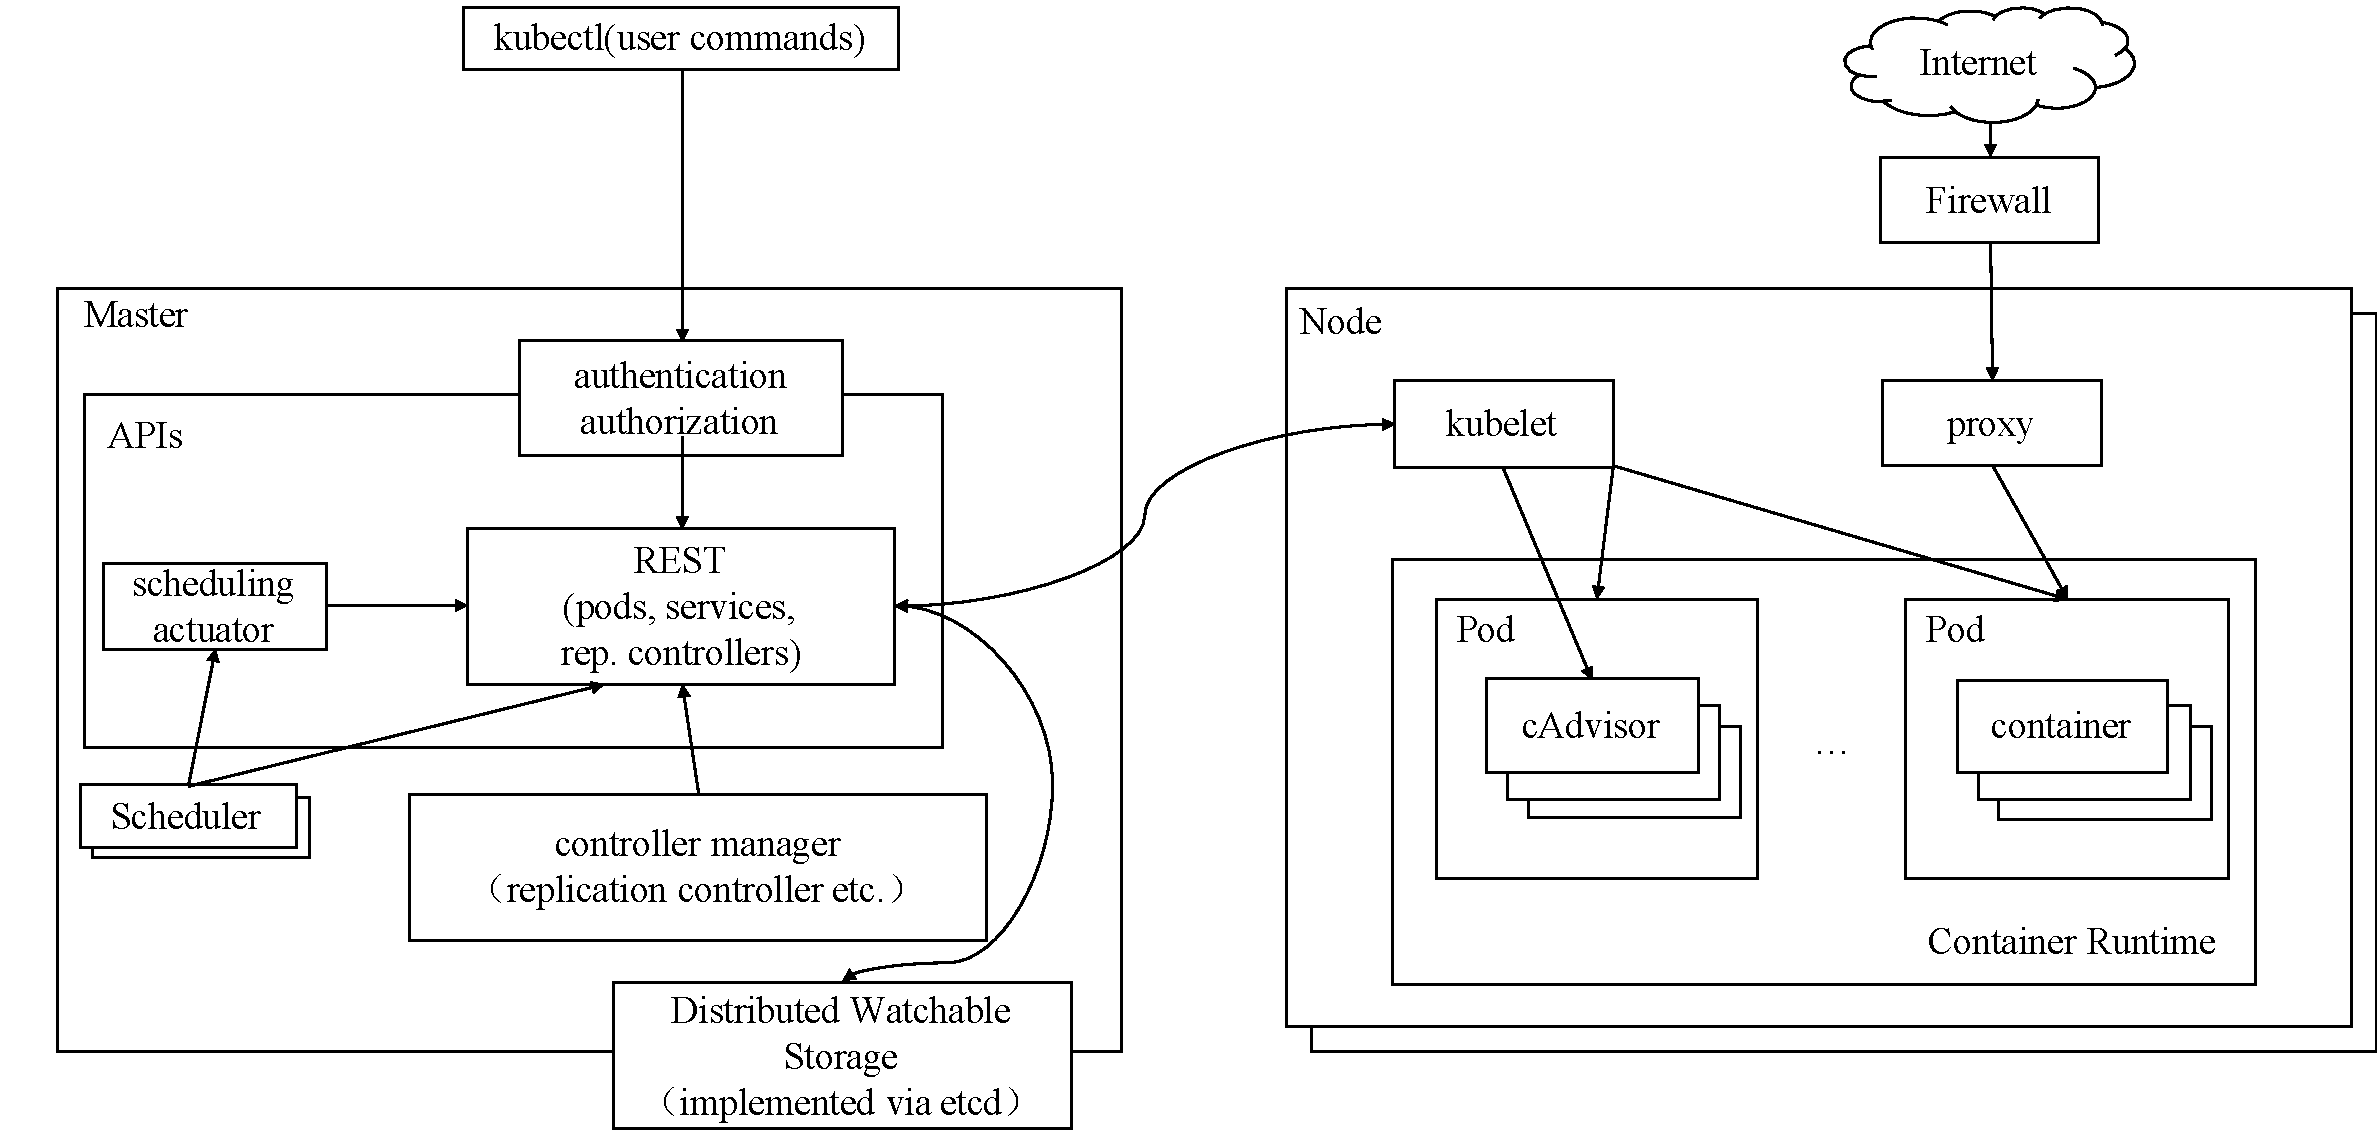
\includegraphics[width=1.0\textwidth]{FIGs/chapter2/k8s.pdf} %中括号中的参数是设置图片充满文档的大小,你也可以使用小数来缩小图片的尺寸。
    \caption{Kubernetes架构图} %caption是用来给图片加上图题的
    \label{k8s} %这是添加标签,方便在文章中引用图片。
\end{figure}%figure环境

Kubernetes由节点代理(kubelet)和Master节点组成。如图\ref{k8s}所示, Kubernetes节点主要由以下核心组件构成:

\begin{itemize}[itemindent=2em]
    \item Etcd: 用于保存集群中一切网络配置和状态信息;

    \item APIServer: 是资源配额控制的入口, 具备完备的集群安全机制并且提供用于集群管理的REST API接口;

    \item Controller Manager: 集群内部的所有资源的管理控制中心, 负责集群内的Node、Pod副本、Endpoint、Namespace、ServiceAccount、ResourceQuota的管理, 实现自动扩展、自动滚动更新、故障检测等功能;

    \item Sheduler: 根据特定的调度算法将Pod调度到指定的工作节点;

    \item kubelet: 定时检查获取节点上Pod、容器的期望状态, 并调用对应的容器平台接口达到这个状态;

    \item Container Runtime: 负责镜像管理以及Pod和容器的真正运作\cite{wangjunxiang2018};

    \item kube-proxy: 为Service提供集群内部的负载均衡和服务发现。
\end{itemize}

Kubernetes拥有独特的声明式API设计, 即声明式地告诉Kubernetes所需资源的状态, 而不是告诉它如何做。在Kubernetes中对象(Object)是持久化的实体, Kubernetes使用这些实体去表示整个集群的状态, 同时这些对象可以在Yaml\cite{ben2009yaml}文件中作为一种声明式API类型来灵活地创建并配置。典型的, Kubernetes的对象主要有以下几种: 

\begin{itemize}[itemindent=2em]
    \item Namespace: 能够隔离资源。Kubernetes集群可以拥有多个命名空间, 这些命名空间在逻辑上彼此隔离, 实现了对多用户的资源隔离;

    \item Pod: Kubernetes中最基本的操作单元, 包含一个或多个容器。Kubernetes为每个Pod分配一个唯一的IP地址, Pod内部的多个容器共享该IP地址。并且每个Pod都能设定自己的计算资源, 即CPU和Memory;

    \item Replication Controller(简称RC): 确保任意时间Kubernetes集群中运行指定数量的Pod副本;

    \item Deployment: 保证Pod的数量和健康, 绝大多数的功能与RC完全一样, 能够被当作全新一代的RC;

    \item Service: 定义了一个Pod逻辑集合以及访问Pod的策略, 它提供一种桥梁会为访问者提供一个固定的Pod访问地址用于在访问时重定向到相应的后端;

    \item Label: 通过键值对的方式被附加到任何资源对象上, 用于配置资源;

    \item Secret: 不需要将敏感数据外露, 解决密码、Token、密钥等敏感数据的配置问题;

    \item Role: 一组权限的集合, 给某个NameSpace中的资源进行鉴权;

    \item ConfigMap: 为了让镜像和配置文件解耦, 应用程序会从配置文件、命令行参数或环境变量中读取配置信息,以便实现镜像的可移植性和可复用性;

    \item Volume: Pod中能够被多个容器访问的持久化共享目录;

    \item Persistent Volume(简称PV): 类似于Volume, Kubernetes提供的存储资源的抽象管理集群存储, 其API内包含存储的细节实现;

    \item Persistent Volume Claim(简称PVC): 对存储资源的请求声明, PVC不关心底层存储实现的细节, 只消耗PV资源。

\end{itemize}

随着Kubernetes生态的持续发展, 上述常规的资源类型仅代表通用的对象, 并不能适应多变的业务需求。为提升自身的扩展能力, Kubernetes提供用户自定义CRD向Kubernetes API中增加定制化的资源类型。用户的自定义资源(Custom Resource, 简称CR)创建并注册到Kubernetes API后, 其与常规通用资源对象都是原生的、存在于etcd中的同等资源, 可以采用Kubernetes原生方式进行创建、查看。CRD本质上用于声明用户自定义资源对象, 开发人员还需要针对CRD提供关联的Operator对CR进行完整生命周期管控。

Operator主要负责有状态应用(即CR)及其组件的部署、更新、自动扩展、维护、数据备份等, 保证它们的可用性。Operator作为Kubernetes的一种扩展形式, 基于Kubernetes的资源和控制器(Controller)概念构建, 遵循Kubernetes原则, 功能类似于Controller Manager, 但同时又注入了特定领域知识。

% \section{其他相关技术}\label{section: other_technologies}

\section{Helm}\label{section: other_technologies}

Helm是一种基于Kubernetes云计算平台的打包和部署复杂软件应用程序的技术\cite{spillner2019quality}。随着云原生及微服务架构的发展, 开发人员倾向于将大的单体应用分解成多个可以独立开发、部署、运维的微服务部署于Kubernetes之上。服务数量的增加为Kubernetes编排带来了复杂性, Helm则通过软件打包的方式极大地简化了Kubernetes应用部署和管理的复杂性。

Helm存在三个核心概念:

\begin{itemize}[itemindent=2em]
    \item chart: 即一系列包含创建Kubernetes应用实例必要信息的文件;

    \item config: 包含应用发布的相关配置信息;

    \item release: chart及其配置的运行实例。
\end{itemize}

如图\ref{helm}所示, Helm将Kubernetes资源(如Deployment、Service)打包到chart中, chart将会被保存到仓库中。Tiller是部署于Kubernetes中的Helm的服务端, 负责接受Helm请求并于APIServer进行交互, 根据chart生成并管理release。开发者使用Helm可以简化应用配置及版本管理, 使得在Kubernetes上部署、升级、回滚、卸载应用程序更加方便。

\begin{figure}[h] %figure环境,h默认参数是可以浮动,不是固定在当前位置。如果要不浮动,你就可以使用大写float宏包的H参数,固定图片在当前位置,禁止浮动。
    \centering %使图片居中显示
    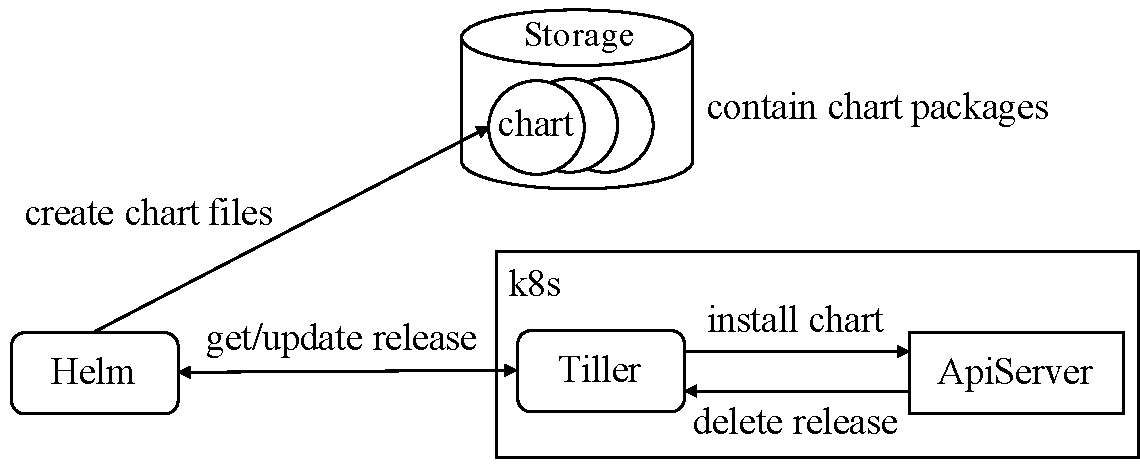
\includegraphics[width=0.8\textwidth]{FIGs/chapter2/helm.pdf} %中括号中的参数是设置图片充满文档的大小,你也可以使用小数来缩小图片的尺寸。
    \caption{Helm架构图} %caption是用来给图片加上图题的
    \label{helm} %这是添加标签,方便在文章中引用图片。
\end{figure}%figure环境

% \subsection{Istio}

% 随着技术下沉, 传统由软件本身负责的负载均衡、路由等功能下沉到云原生基础设施。服务网格(Service Mesh)通过在不断变化的条件和拓扑结构面前强制执行所需的网络行为, 为网络连接的工作负载提供基于策略的网络服务\cite{calcote2019istio}。Istio\footnotemark[1]\footnotetext[1]{\href{https://github.com/istio/istio}{istio}}是Service Mesh架构的一种实现方式, 其是一个用于保证容器服务间连接、安全、控制和观测的网络代理组件, 具有负载均衡、服务间认证、监控等功能。

% Istio分为两个逻辑部分\cite{larsson2020impact}: 数据平面(Data Plane)与控制平面(Control Plane)。数据平面由代理程序Envoy(通常被称为Sidercar)组成, 其受控制平面组件控制, 通常与业务容器捆绑, 来劫持业务应用容器的流量完成针对特性应用程序的控制与治理; 控制平面提供服务发现、配置和证书管理等功能, Istio对其进行了进一步细分:

% \begin{itemize}[itemindent=2em]
%     \item Mixer: 负责策略、访问控制和请求追踪;

%     \item Pilot: 提供服务发现的功能;

%     \item Citadel: 负责证书颁发;
% \end{itemize}

\section{本章小结}

本章第\ref{section: blockchain}节首先介绍了区块链基本概念、架构、分类, 其次重点介绍联盟链解决方案HF的网络节点、账本结构, 最后介绍区块链即服务的诞生和通用架构; 第\ref{section: cloud_native}节介绍云原生的发展历程、技术范畴以及Kubernetes; 第\ref{section: other_technologies}节介绍本文区块链云化框架涉及到的其他相关技术。

% \begin{figure}[!htbp] %figure环境,h默认参数是可以浮动,不是固定在当前位置。如果要不浮动,你就可以使用大写float宏包的H参数,固定图片在当前位置,禁止浮动。
%     \centering %使图片居中显示
%     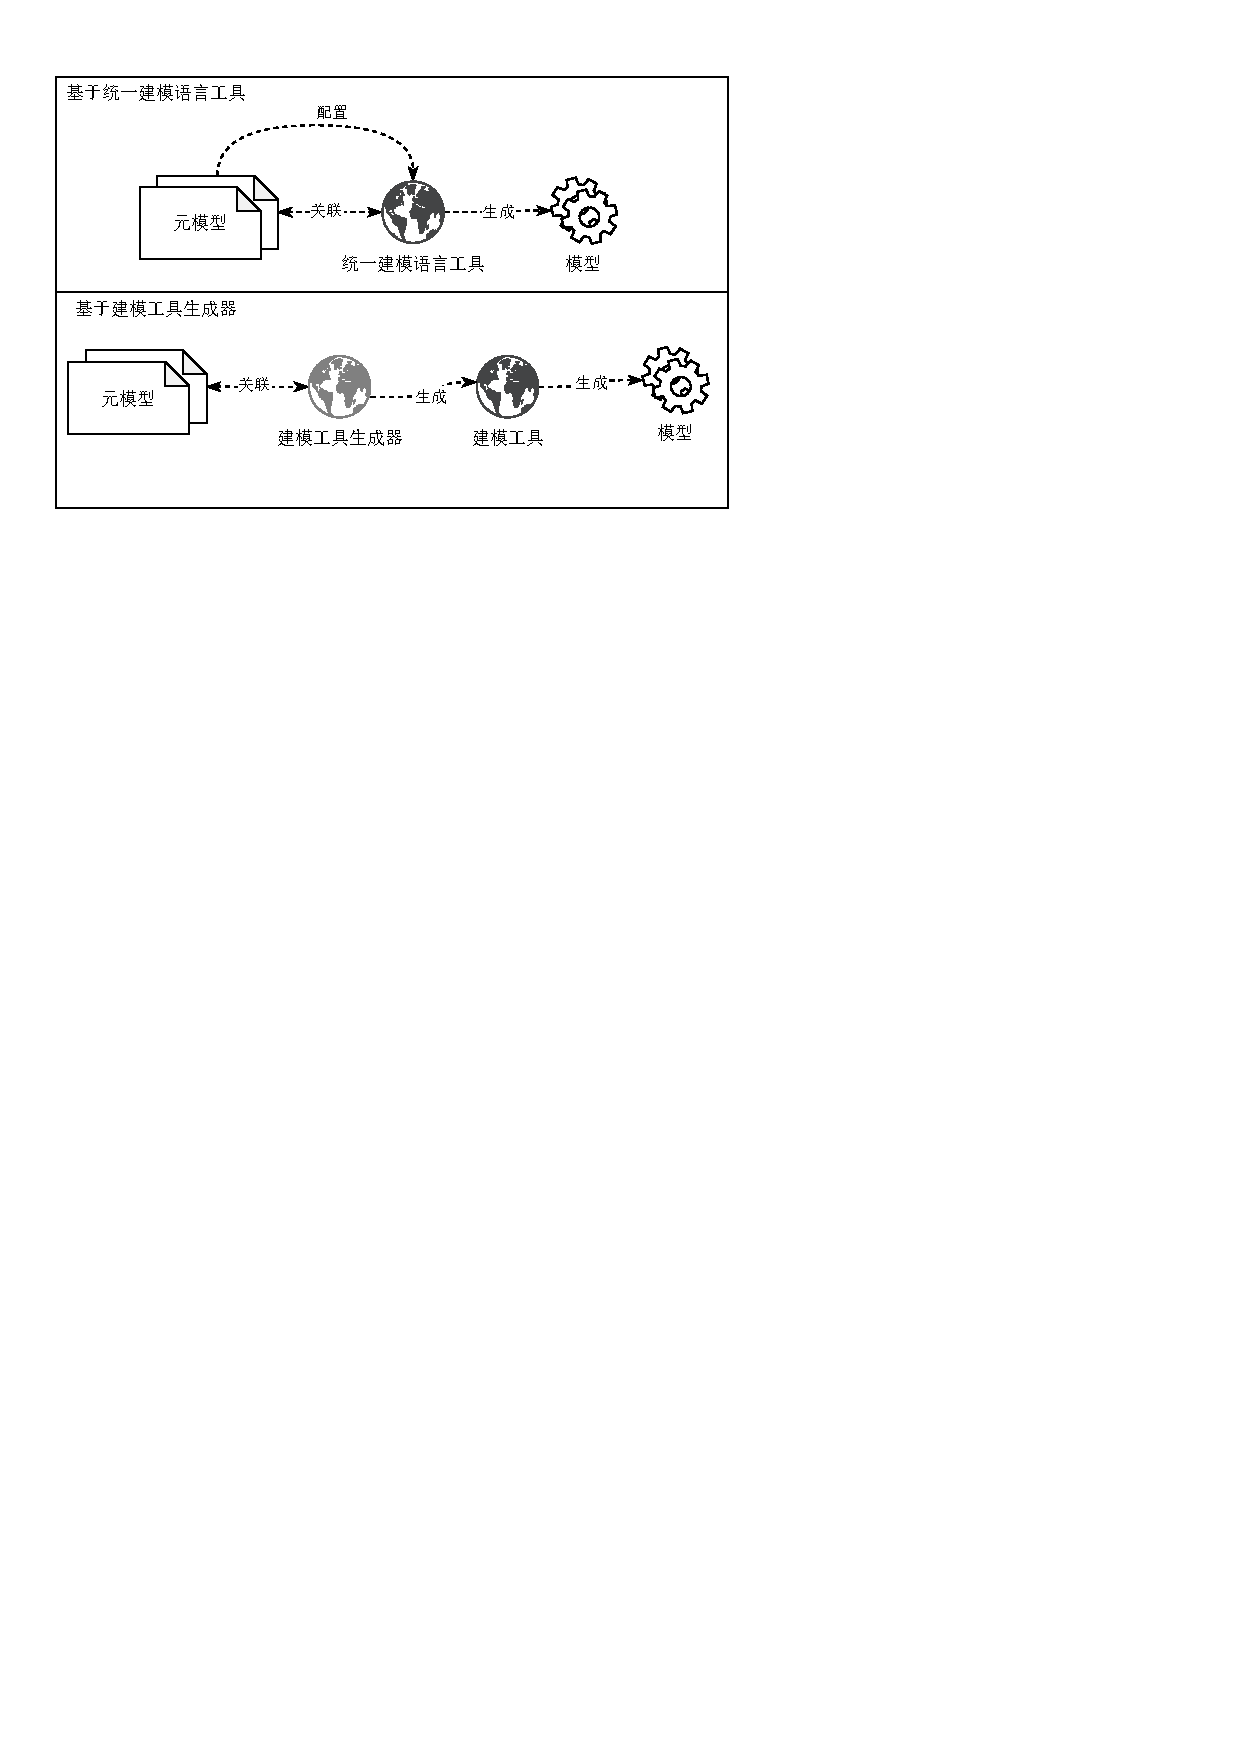
\includegraphics[width=0.8\textwidth]{FIGs/chapter3/2kindsmodeling.pdf} %中括号中的参数是设置图片充满文档的大小,你也可以使用小数来缩小图片的尺寸。
%     \caption{两种建模工具实施方式} %caption是用来给图片加上图题的
%     \label{2kindsmodeling} %这是添加标签,方便在文章中引用图片。
% \end{figure}%figure环境





